The reference systems used throughout the project are explained below: 

\begin{itemize}

\item Body frame (B): 

These axes are continuously fixed to the aircraft, with their origin situated in the airplane's center of mass. The x-axis is contained in the airplane's symmetry plane and is pointing towards the front of the aircraft. The z-axis is also contained in the aircraft's symmetry plane and is pointing towards the bottom of the aircraft, being perpendicular to the x-axis. Meanwhile, the y-axis forms a right-handed trihedron with the other two axis, and points towards the right semi-span. This frame is represented in figure \ref{fig:B_frame}.

\begin{figure}
\centering
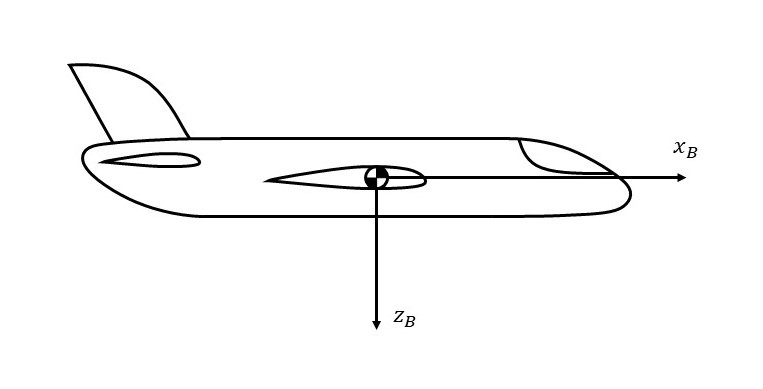
\includegraphics[scale=0.4]{Images/B_frame.jpg}
\caption{Representation of the body frame of reference}
\label{fig:B_frame}
\end{figure}

\item Wind frame (W):

These axes are also centered in the aircraft's center of mass. The x-axis is parallel to the aerodynamic velocity vector of the airplane and has the same direction. The z-axis is contained in the aircraft's symmetry plane and is pointing towards the bottom of the aircraft, being perpendicular to the x-axis. The y-axis forms a right-handed thriedron with the last two axis. This frame is represented in figure \ref{fig:W_frame}.

\begin{figure}
\centering
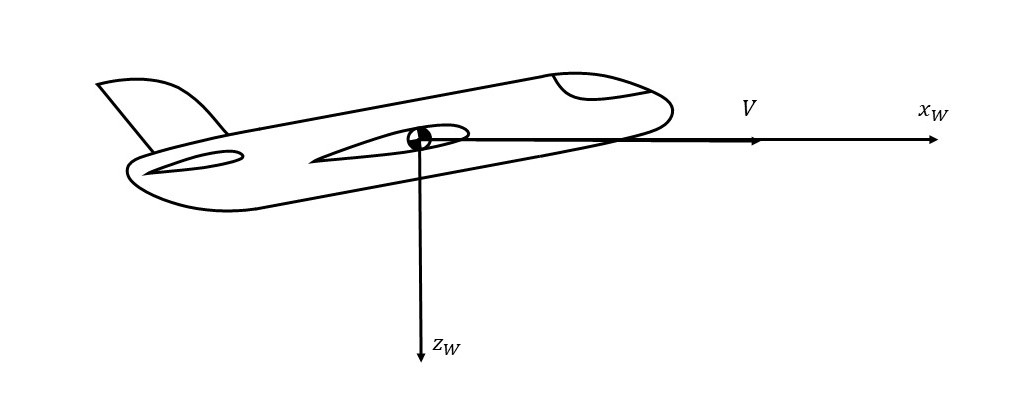
\includegraphics[scale=0.4]{Images/W_frame.jpg}
\caption{Representation of the wind frame of reference}
\label{fig:W_frame}
\end{figure}

\newpage

\item Thrust frame:

These axes are defined the same way as the wind axes, but the x-axis is parallel to the thrust vector and points towards the same direction. This frame is represented in figure \ref{fig:T_frame}.

\begin{figure}
\centering
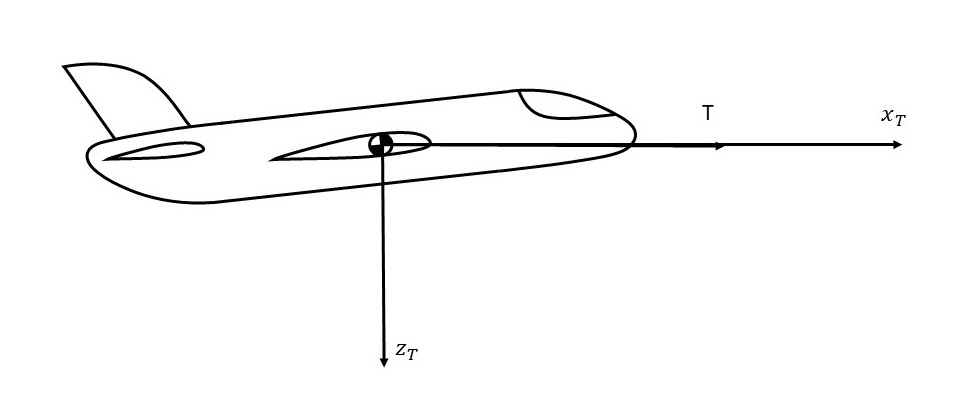
\includegraphics[scale=0.4]{Images/T_frame.jpg}
\caption{Representation of the thrust frame of reference}
\label{fig:T_frame}
\end{figure}

\item Flat Earth frame (FE):

These axes have their origin in the surface point below the initial position of the aircraft. The x axis points towards the initial direction of the aircraft projected on the horizontal plane. The z axis is perpendicular to that horizontal plane and points towards the center of the Earth (below the horizontal plane, considering that a flat Earth would not have a center). The y-axis forms a right-handed thriedron with the last two axis. This way, the position of the aircraft in this frame at t=0 seconds would be $[0, 0, -h_0]$. This frame is represented in figure \ref{fig:FE_frame}.

\begin{figure}
\centering
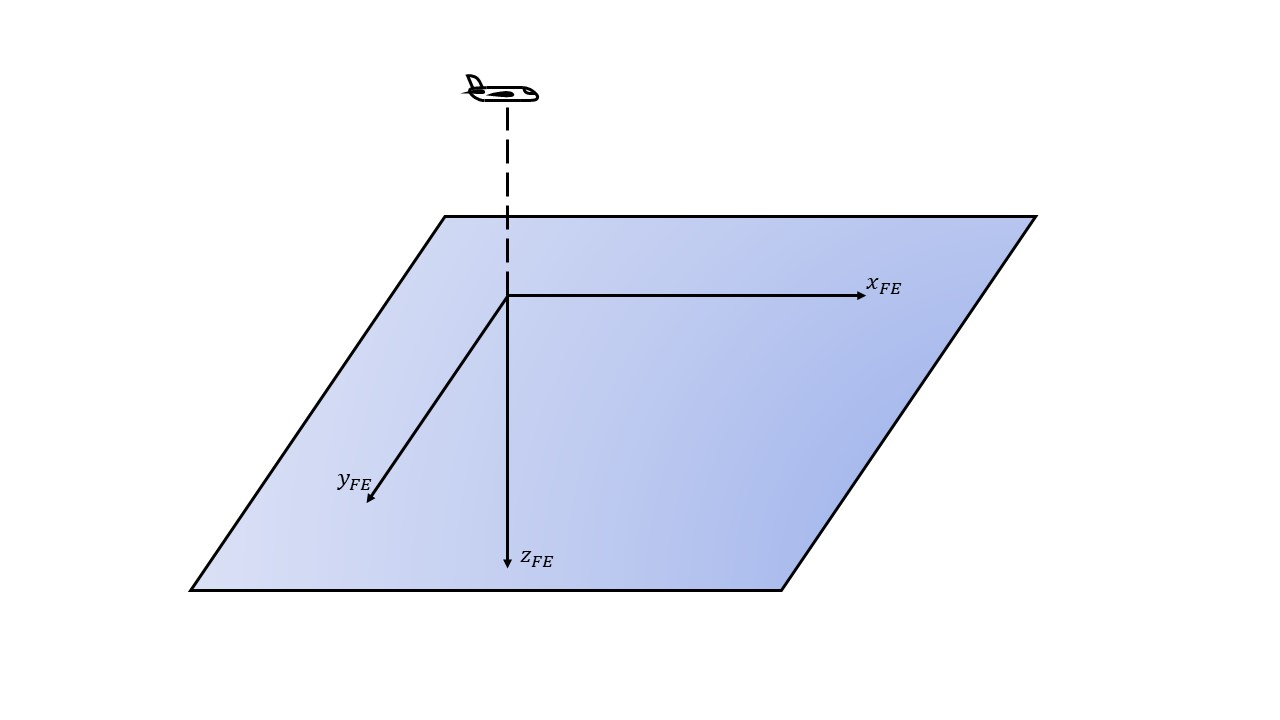
\includegraphics[scale=0.4]{Images/FE_frame.jpg}
\caption{Representation of the flat Earth frame of reference}
\label{fig:FE_frame}
\end{figure}

\item Local Horizon frame (LH):

These axes have their origin at the same point as the Flat Earth axes and share the same z-axis, but the x-axis is oriented towards the north of the Earth and the y-axis points towards the East. This frame is represented in figure \ref{fig:LH_frame}.

\begin{figure}
\centering
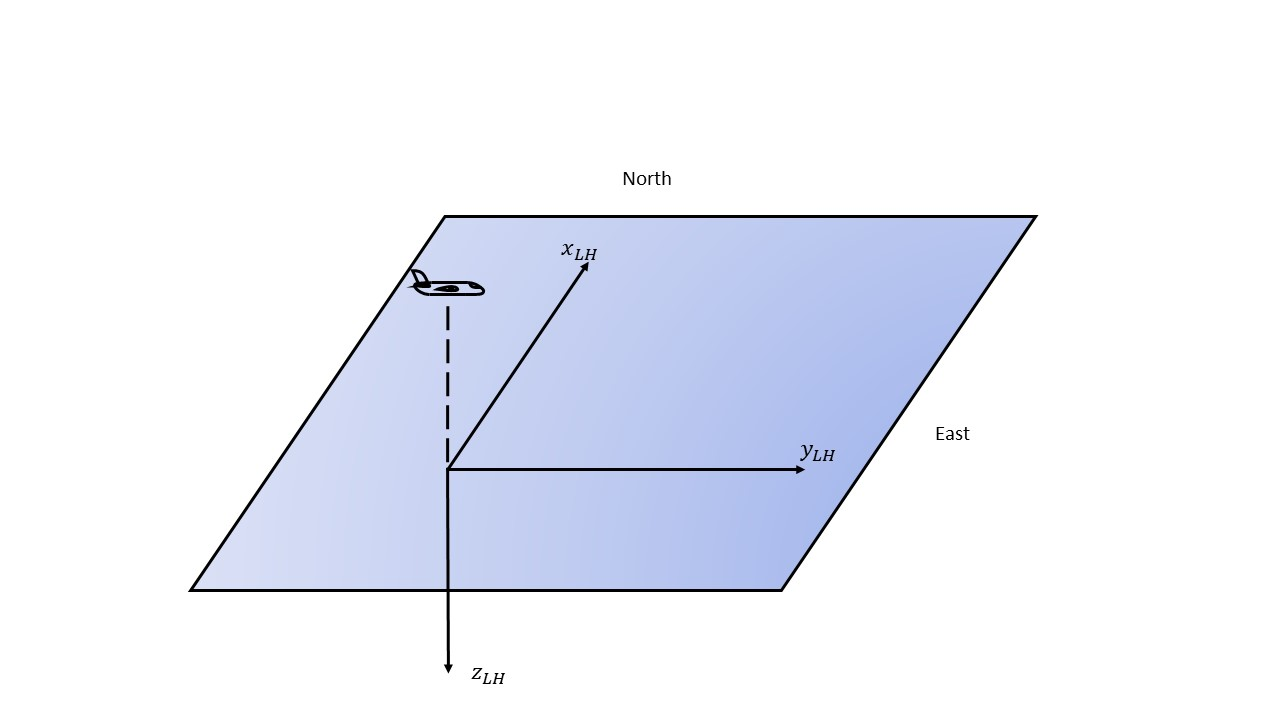
\includegraphics[scale=0.4]{Images/LH_frame.jpg}
\caption{Representation of the local horizon frame of reference}
\label{fig:LH_frame}
\end{figure} 

\newpage

\item Earth Centered Fixed Intermediate frame (ECFI): 

These axis are centered in the Earth's ellipsoid center and rotate with the Earth. The z-axis is parallel to the Earth's rotation axis. The x-axis is always contained in the same plane as the z-axis and the initial position, it is perpendicular to the z-axis and points towards that initial point. The y-axis forms a right-handed thriedron with the last two axis. This frame is represented in figure \ref{fig:ECFI_frame}.

\begin{figure}
\centering
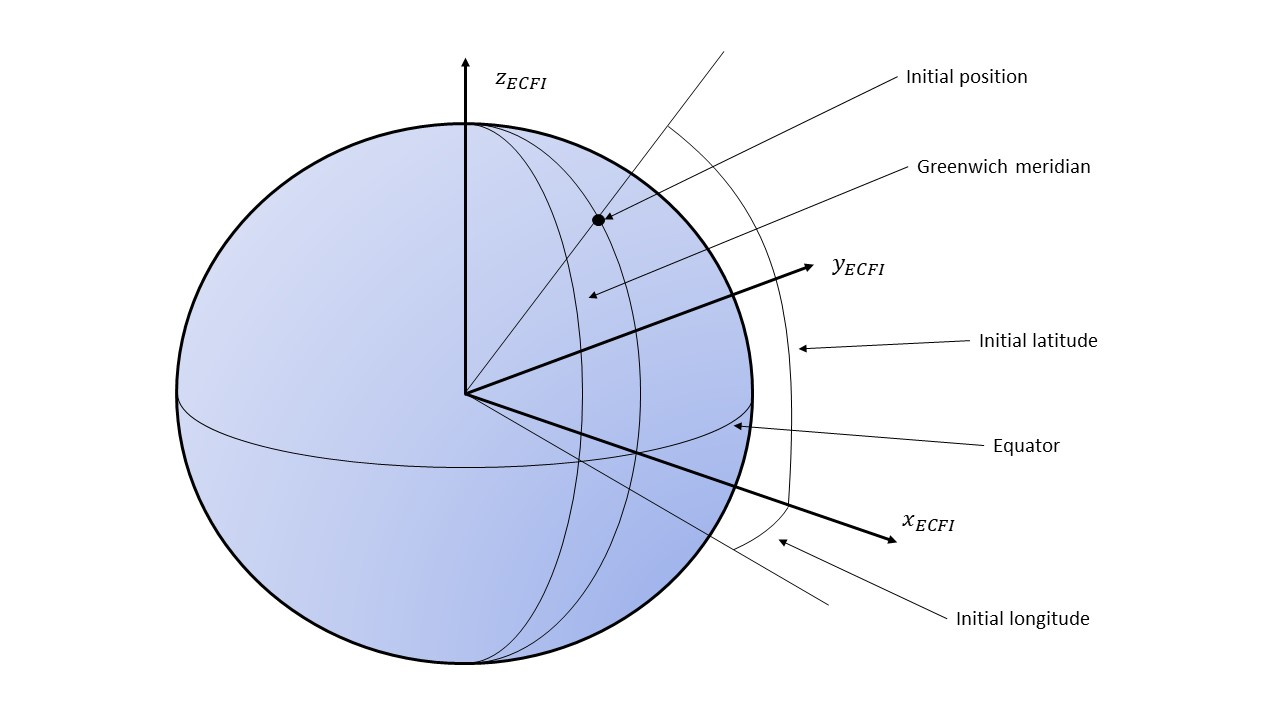
\includegraphics[scale=0.4]{Images/ECFI_frame.jpg}
\caption{Representation of the Earth centered fixed intermediate frame of reference}
\label{fig:ECFI_frame}
\end{figure}

\item Earth Centered Fixed frame (ECF): 

These axes are just like the ECFI ones, but the x-axis always points towards the Greenwich Meridian (latitude 0) instead of pointing towards the initial position of the plane. These axes rotate with the Earth, just like the ECFI axes. This frame is represented in figure \ref{fig:ECF_frame}.

\begin{figure}
\centering
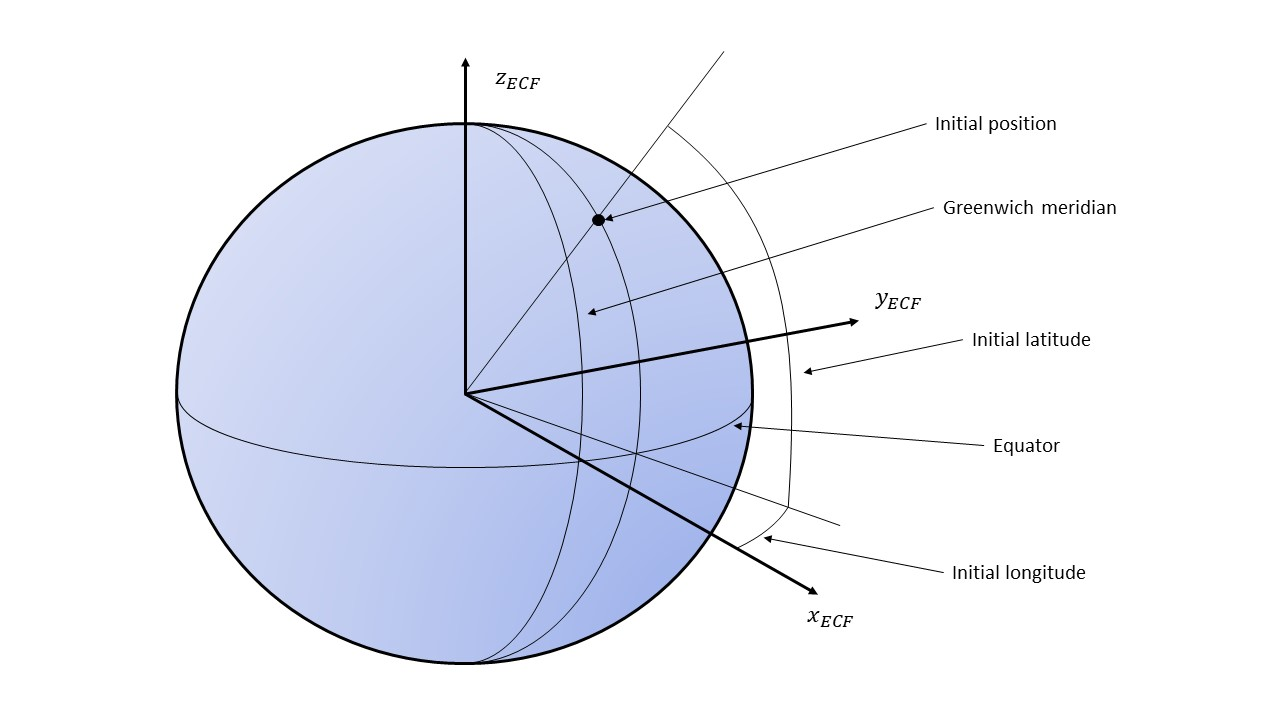
\includegraphics[scale=0.4]{Images/ECF_frame.jpg}
\caption{Representation of the Earth centered fixed frame of reference}
\label{fig:ECF_frame}
\end{figure}

\item Earth Centered Inertial frame (ECI): 

These axes are similar to the ECF axes, but are not fixed to the Earth. The x-axis points towards the Earth's mean equinox, which is the intersection between the equatorial and ecliptic planes, while the z-axis is parallel to the Earth's rotation axis and points towards the north, and the y-axis forms a right handed thriedron with the other axis. This frame is represented in figure \ref{fig:ECI_frame}. 

\begin{figure}
\centering
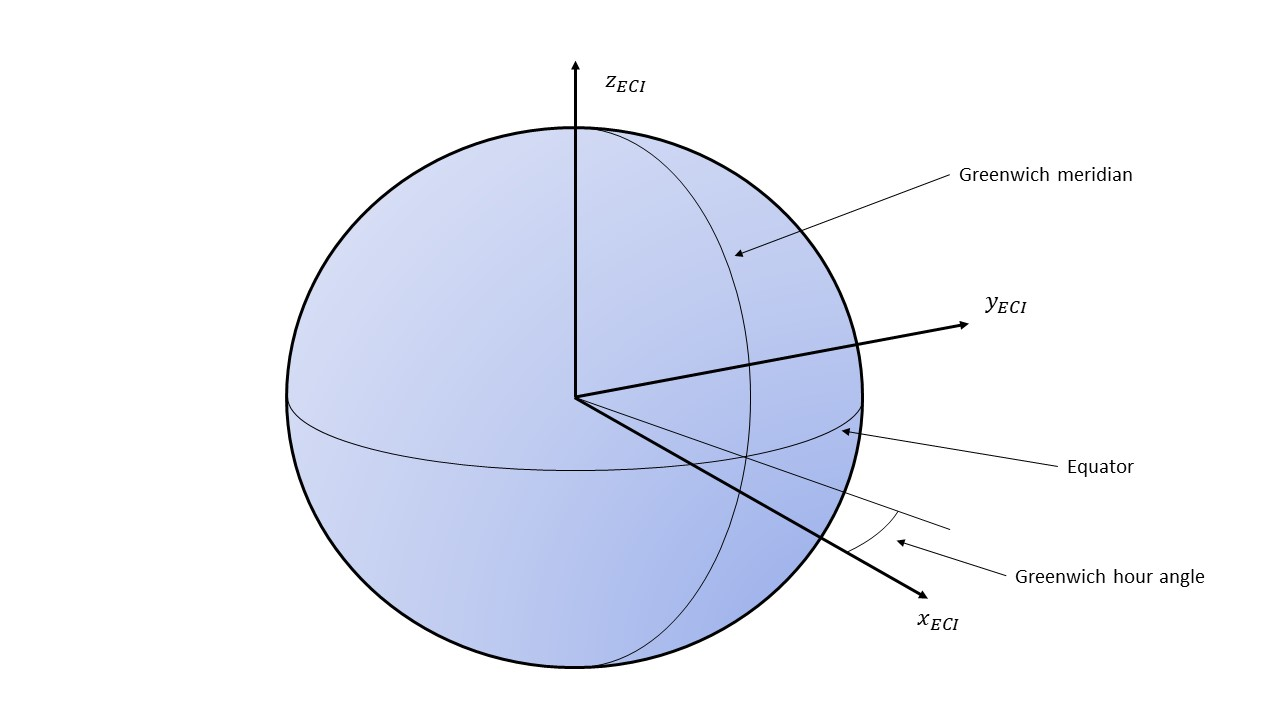
\includegraphics[scale=0.4]{Images/ECI_frame.jpg}
\caption{Representation of the Earth centered inertial frame of reference}
\label{fig:ECI_frame}
\end{figure}

\end{itemize}
